\documentclass{beamer}

\usepackage{epsfig}
\usepackage{multicol}
\usepackage{geometry}
%\usepackage[dvipsnames]{xcolor}
\usepackage{textcomp}
\usepackage{graphicx}
\usepackage{caption}
\usepackage{subcaption}
\usepackage{amsmath}
\usepackage{tcolorbox}
\usetheme{Boadilla}
\usepackage{pict2e}
\usepackage{tikz}
\usepackage{xcolor}

\usetikzlibrary {decorations.pathmorphing}

\title[Traitement du signal numérique]{Traitement du signal numérique - HEI4 IMS}
\author[Antony Bazir]{}

\setlength{\unitlength}{1cm}

\begin{document}
\section{Application Doppler embolie}
\begin{frame} 
\frametitle{Détection d'embolie gazeuse dans les veines}
\begin{center}
\includegraphics[scale=0.5]{gaseous_emboli.png}\\
\textit{\footnotesize P. Marsh, 2023, Frontiers}
\end{center}
\underline{Origines principales} : 
\begin{itemize}
\item \textbf{Iatrogéniques} : geste médical ou chirurgical 
\item \textbf{Accident de décompression} : plongée, environnement haute pression, etc...
\end{itemize}
\end{frame} 

\begin{frame} 
\frametitle{Détection d'embolie gazeuse dans les veines}
\begin{center}
\includegraphics[scale=0.5]{gaseous_emboli.png}\\
\textit{\footnotesize P. Marsh, 2023, Frontiers}
\end{center}
\underline{Problèmes} : 
\begin{itemize}
\item Bulles stables $\rightarrow$ circulation dans le système sanguin
\item Potentielle atteinte organes vitaux (coeur, poumons)
\end{itemize}
\end{frame} 

\begin{frame} 
\frametitle{Détection d'embolie gazeuse dans les veines}
\begin{center}
\includegraphics[scale=0.5]{gaseous_emboli.png}\\
\textit{\footnotesize P. Marsh, 2023, Frontiers}
\end{center}
\underline{Caractéristiques des bulles}
\begin{itemize}
\item diamètre: 8 - 700 \textmu m
\item "gamme de densité" :  1-100
\end{itemize}
\end{frame}

\begin{frame} 
\frametitle{Détection d'embolie gazeuse dans les veines}
\begin{center}
\includegraphics[scale=0.5]{gaseous_emboli.png}\\
\textit{P. Marsh, 2023, Frontiers}
\end{center}
\textbf{Détecter les bulles ?}
\begin{itemize}
\item Méthode non-invasive
\item Mécanisme physique générant un bon rapport signal/bruit
\item Résolution spatiale et temporelle suffisantes
\end{itemize}

\end{frame} 

\begin{frame}
\frametitle{Méthodes de détection possibles des embolies gazeuses}
\begin{center}
\includegraphics[scale=0.5]{gaseous_emboli.png}\\
\textit{P. Marsh, 2023, Frontiers}
\end{center}
\vspace{0.1cm}
\underline{Familles de techniques} :
\vspace{0.1cm}
\begin{itemize}
\item \textbf{Techniques acoustiques} : basées sur la réflectivité importante des bulles 
\vspace{0.1cm}
\item \textbf{Technique optiques} : basées sur l'interface optique bulle/sang
\vspace{0.1cm}
\item \textbf{IRM }: Utilisé surtout pour le cerveau
\end{itemize}

\end{frame}

\begin{frame}
\frametitle{Détection ultrasonore des embolies veineuses gazeuses}
\begin{center}
\usetikzlibrary {decorations.pathmorphing}
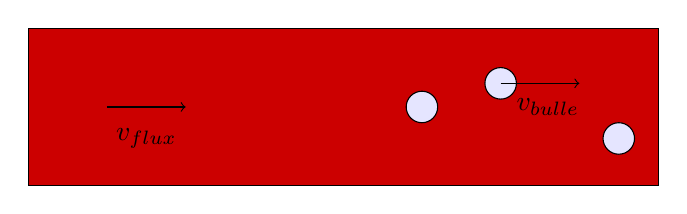
\begin{tikzpicture}
\draw[fill=red!80!black] (0,0) rectangle (8,2);
\draw[fill=blue!10!white] (5,1) circle(0.2) ;
\draw[fill=blue!10!white] (6,1.3) circle(0.2) ;
\draw[fill=blue!10!white] (7.5,0.6) circle(0.2) ;
\draw[->] (1,1)--(2,1);
\draw (1.5, 0.6) node[text centered] {$v_{flux}$};
\draw[->] (6,1.3)--(7,1.3);
\draw (6.6, 1) node[text centered] {$v_{bulle}$};
\end{tikzpicture}
\end{center}
\vspace{0.1cm}
\underline{Infos disponible} :
\vspace{0.1cm}
\begin{itemize}
\item \textbf{Sang} :  $c_{sang}$ = 1580 m/s et $\rho_{sang} $  = 1060 kg/m$^3$ 
\vspace{0.2cm}
\item \textbf{Bulle} :  $c_{bulle}$ = 330 m/s et $\rho_{sang} $  = 1.18 kg/m$^3$ 
\vspace{0.2cm}
\item \textbf{Vitesse} : $\bar{v_{bulle}}$ $\approx$ $\bar{v_{flux}}$
\end{itemize}

\end{frame}

\begin{frame}
\frametitle{Détection ultrasonore des embolies veineuses gazeuses}
Interaction onde acoustique/vaisseau sanguin+bulles:

\begin{center}
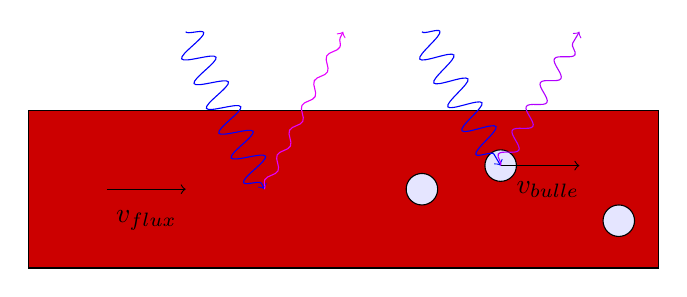
\begin{tikzpicture}
\draw[fill=red!80!black] (0,0) rectangle (8,2);
\draw[fill=blue!10!white] (5,1) circle(0.2) ;
\draw[fill=blue!10!white] (6,1.3) circle(0.2) ;
\draw[fill=blue!10!white] (7.5,0.6) circle(0.2) ;
\draw[->] (1,1)--(2,1);
\draw (1.5, 0.6) node[text centered] {$v_{flux}$};
\draw[->] (6,1.3)--(7,1.3);
\draw (6.6, 1) node[text centered] {$v_{bulle}$};

 \draw [->,decorate,decoration={snake,amplitude=2mm},blue] (2,3) -- (3,1);
  \draw [->,decorate,decoration={snake,amplitude=0.5mm},blue!10!magenta] (3,1) -- (4,3);
  
   \draw [->,decorate,decoration={snake,amplitude=2mm},blue] (5,3) -- (6,1.3);
  \draw [->,decorate,decoration={snake,amplitude=1mm},blue!30!magenta] (6,1.3) -- (7,3);
\end{tikzpicture}
\end{center}
\vspace{0.1cm}
\begin{itemize}
\item $\bar{v_{bulle}}$ $\approx$ $\bar{v_{flux}}$ $\rightarrow$ $\Delta f_{bulle}$ $\approx$ $\Delta f_{flux}$ $\rightarrow$ fréquence Doppler inadaptée
\vspace{0.2cm}
\item $c_{sang} \rho_{sang}$ $>>$ $c_{bulle} \rho_{bulle}$ $\rightarrow$  forte réflexion à l'interface bulle/sang
\end{itemize}
\vspace{0.2cm}
\textbf{Recherche de bulles = Recherche de fortes amplitudes}


\end{frame}

\begin{frame}
\frametitle{Détection ultrasonore des embolies veineuses gazeuses}
\'Etude de Pierleoni \textit{et al.}, MDPI, 2019
\begin{columns}
\column{60mm}
\begin{center}
\includegraphics[scale=0.3]{precordium.png}\\
\textit{\footnotesize Jagelavicius et al., PJCT, 2013}
\end{center}
\column{60mm}
\underline{Mesures signaux ultrasonore} :
\vspace{0.2cm}
\begin{itemize}
\item Cohorte de plongeurs 
\vspace{0.2cm}
\item Sonde Ultrason Doppler 2 MHz
\vspace{0.2cm}
\item Sondage dans la zone précordiale 
\end{itemize}
\end{columns}

\end{frame}

\begin{frame}
\frametitle{Détection ultrasonore des embolies veineuses gazeuses}
\'Etude de Pierleoni \textit{et al.}, MDPI, 2019

\begin{center}
\includegraphics[scale=0.4]{extrait_signal.png}\\
\textit{\footnotesize Extrait d'un signal brut enregistré sur un plongeur}
\end{center}


\begin{itemize}
\item Artefacts de positionnement de la sonde  
\vspace{0.1cm}
\item Zone de pause 
\vspace{0.1cm}
\end{itemize}

$\rightarrow$ pré-traitement temporel pour enlever les artefacts

\end{frame}

\begin{frame}
\frametitle{Détection ultrasonore des embolies veineuses gazeuses}
\'Etude de Pierleoni \textit{et al.}, MDPI, 2019

\begin{center}
\includegraphics[scale=0.4]{signal_pretraite.png}\\
\textit{\footnotesize Signal prétraité}
\end{center}


\begin{itemize}
\item Comment distinguer les bulles du bruit de fond ?  
\end{itemize}

\end{frame}

\begin{frame}
\frametitle{Détection ultrasonore des embolies veineuses gazeuses}
\'Etude de Pierleoni \textit{et al.}, MDPI, 2019

\begin{columns}
\column{60mm}
\begin{center}
\includegraphics[scale=0.25]{signal_pretraite.png}\\
\textit{\footnotesize Signal prétraité}
\end{center}

\column{60mm}
\begin{itemize}
\item Signal aléatoire en apparence
\vspace{0.2cm} 
\item 2 composantes :
\vspace{0.1cm}
\begin{itemize}
\item \textbf{bruit de fond} : non stationnaire, quasi-périodique
\vspace{0.1cm}
\item \textbf{bulle} : non stationnaire, transitoire
\vspace{0.1cm}
\end{itemize}
\end{itemize}
\vspace{0.2cm}
$\rightarrow$ Outils d'analyse processus non-stationnaire... 
\end{columns}

\end{frame}

\begin{frame}
\frametitle{Détection ultrasonore des embolies veineuses gazeuses}

\textbf{\underline{Objectif}: Séparer la composante transitoire et la composante quasi-périodique}\\

\vspace{0.5cm}
Méthode proposée par Pierleoni et al. : \underline{Décomposition de mode empirique}
\vspace{0.2cm}
\begin{itemize}
\item Signal = somme de \textbf{fonctions de mode intrinsèques (FMI)}
\vspace{0.2cm}
\item Deduction \textbf{itérative} des FMI 
\vspace{0.2cm}
\item 1eres composantes = hautes fréquences $\rightarrow$ dernières composantes = basses fréquences

\end{itemize}

\end{frame}

\begin{frame}
\frametitle{Détection ultrasonore des embolies veineuses gazeuses}


\underline{\'Etapes de la méthode de Pierleoni et al.}
\vspace{0.2cm}
\begin{enumerate}
\item Extraction de tous les \textbf{extrema} du signal prétraité
\vspace{0.2cm}
\item Formation des enveloppes $e_{min}(t)$ et $e_{max}(t)$ par interpolation des minima et maxima
\vspace{0.2cm}
\item Calculer $r(t) = \frac{\displaystyle e_{min} + e_{max}}{\displaystyle 2}$
\vspace{0.2cm}
\item Calculer $c(t) = x(t) - r(t)$
\vspace{0.2cm}
\item Répéter 5 fois les pas 1 à 4 
\vspace{0.2cm}
\item Diviser $c(t)$  en bandes de 10 ms et extraire pour chacune le maximum en amplitude
\item Comparer ces maxima à un seuil et conclure sur la présence/non-présence de bulles
\end{enumerate}

\end{frame}

\begin{frame}
\frametitle{Détection ultrasonore des embolies veineuses gazeuses}
Extrait de signal brut :
\begin{center}
\begin{tikzpicture}
\begin{scope}[scale=2.5]
\draw[->] (0,0)-- (2.1,0)node[right] {\scriptsize $t$} ;
\draw[->] (0,-0.6)-- (0,0.6)node[above] {\scriptsize  $s(t)$};
\draw[thick,blue] plot file {raw_sig.txt};

\draw[dashed] (2,0) node[below right]{\scriptsize 22 ms}--(2,0);
\end{scope}

\end{tikzpicture}
\end{center}

\end{frame}

\begin{frame}
\frametitle{Détection ultrasonore des embolies veineuses gazeuses}
\underline {\'Etape 1a : Extraction des minima}
\begin{center}
\begin{tikzpicture}
\begin{scope}[scale=2.5]
\draw[->] (0,0)-- (2.1,0)node[right] {\scriptsize $t$} ;
\draw[->] (0,-0.6)-- (0,0.6)node[above] {\scriptsize  $s(t)$};
\draw[thick,blue] plot file {raw_sig.txt};
\draw[thick,green] plot [ycomb] file {minimae.txt};

\draw[dashed] (2,0) node[below right]{\scriptsize 22 ms}--(2,0);
\end{scope}

\end{tikzpicture}
\end{center}

\end{frame}

\begin{frame}
\frametitle{Détection ultrasonore des embolies veineuses gazeuses}
\underline {\'Etape 1b : Extraction des maxima}
\begin{center}
\begin{tikzpicture}
\begin{scope}[scale=2.5]
\draw[->] (0,0)-- (2.1,0)node[right] {\scriptsize $t$} ;
\draw[->] (0,-0.6)-- (0,0.6)node[above] {\scriptsize  $s(t)$};
\draw[thick,blue] plot file {raw_sig.txt};
\draw[thick,red] plot [ycomb] file {maximae.txt};

\draw[dashed] (2,0) node[below right]{\scriptsize 22 ms}--(2,0);
\end{scope}

\end{tikzpicture}
\end{center}

\end{frame}


\begin{frame}
\frametitle{Détection ultrasonore des embolies veineuses gazeuses}
\underline {\'Etape 2 : Interpolation des enveloppes}
\begin{columns}
\column{50mm}
\begin{center}
\begin{tikzpicture}
\begin{scope}[scale=2]
\draw[->] (0,0)-- (2.1,0)node[right] {\scriptsize $t$} ;
\draw[->] (0,-0.6)-- (0,0.6)node[above] {\scriptsize  $s(t)$};
\draw[thick,red] plot [ycomb] file {maximae.txt};

\draw[dashed] (2,0) node[below right]{\scriptsize 22 ms}--(2,0);
\end{scope}

\end{tikzpicture}
\end{center}

\column{10mm}
\begin{center}
\begin{tikzpicture}
\draw[->] (0,0)--(1,0);
\end{tikzpicture}
\end{center}

\column{50mm}
\begin{center}
\begin{tikzpicture}
\begin{scope}[scale=2]
\draw[->] (0,0)-- (2.1,0)node[right] {\scriptsize $t$} ;
\draw[->] (0,-0.6)-- (0,0.6)node[above] {\scriptsize  $s(t)$};
\draw[dashed,red] plot [ycomb] file {maximae.txt};
\draw[thick,red] plot file {e_maximae.txt};
\draw[dashed] (2,0) node[below right]{\scriptsize 22 ms}--(2,0);
\end{scope}

\end{tikzpicture}
\end{center}
\end{columns}
\vspace{0.5cm}
\begin{itemize}
\item Objectif : relier les points pour former une enveloppe
\item Interpolation par splines cubiques
\end{itemize}

\end{frame}



\begin{frame}
\frametitle{Détection ultrasonore des embolies veineuses gazeuses}
\underline {\'Etape 2 : Interpolation des enveloppes}
\begin{columns}
\column{50mm}

\begin{center}
\begin{tikzpicture}
\begin{scope}[scale=1.5]
\draw[->] (0,0)-- (2.1,0)node[right] {\scriptsize $t$} ;
\draw[->] (0,-0.6)-- (0,0.6)node[above] {\scriptsize  $s(t)$};
\draw[thick,blue] plot file {raw_sig.txt};
\draw[thick,green] plot [ycomb] file {minimae.txt};

\draw[dashed] (2,0) node[below right]{\scriptsize 22 ms}--(2,0);
\end{scope}

\end{tikzpicture}
\end{center}

\begin{center}
\begin{tikzpicture}
\begin{scope}[scale=1.5]
\draw[->] (0,0)-- (2.1,0)node[right] {\scriptsize $t$} ;
\draw[->] (0,-0.6)-- (0,0.6)node[above] {\scriptsize  $s(t)$};
\draw[thick,blue] plot file {raw_sig.txt};
\draw[thick,red] plot [ycomb] file {maximae.txt};

\draw[dashed] (2,0) node[below right]{\scriptsize 22 ms}--(2,0);
\end{scope}

\end{tikzpicture}
\end{center}

\column{10mm}
\begin{center}
\begin{tikzpicture}
\draw[->] (0,0)--(1,0);
\end{tikzpicture}
\end{center}


\column{60mm}
\begin{center}
\begin{tikzpicture}
\begin{scope}[scale=2]
\draw[->] (0,0)-- (2.1,0)node[right] {\scriptsize $t$} ;
\draw[->] (0,-0.6)-- (0,0.6)node[above] {\scriptsize  $s(t)$};
\draw[dotted,blue] plot file {raw_sig.txt};
\draw[thick,red] plot file {e_maximae.txt};
\draw[thick,green] plot file {e_minimae.txt};
\draw[dashed] (2,0) node[below right]{\scriptsize 22 ms}--(2,0);
\end{scope}

\end{tikzpicture}
\end{center}
\end{columns}
\vspace{0.3cm}
\begin{itemize}
\item Signal monotone $\rightarrow$ Enveloppes distantes 
\item Petites fluctuations $\rightarrow$ Enveloppes proches
\end{itemize}


\end{frame}

\begin{frame}
\frametitle{Détection ultrasonore des embolies veineuses gazeuses}
\underline {\'Etape 3 : Calcul de la moyenne}
\begin{center}
\begin{tikzpicture}
\begin{scope}[scale=2.5]
\draw[->] (0,0)-- (2.1,0)node[right] {\scriptsize $t$} ;
\draw[->] (0,-0.6)-- (0,0.6)node[above] {\scriptsize  $s(t)$};
\draw[dotted,blue] plot file {raw_sig.txt};
\draw[thick,magenta] plot file {mean.txt};
\draw[dashed] (2,0) node[below right]{\scriptsize 22 ms}--(2,0);
\end{scope}

\end{tikzpicture}
\end{center}
\vspace{0.3cm}
\begin{itemize}
\item Enveloppes distantes $\rightarrow$  Moyenne éloignée du signal
\item Enveloppes proches $\rightarrow$ Moyenne proche du signal
\end{itemize}

\end{frame}

\begin{frame}
\frametitle{Détection ultrasonore des embolies veineuses gazeuses}
\underline {\'Etape 4 : c(t) = x(t)-r(t)}
\begin{center}
\begin{tikzpicture}
\begin{scope}[scale=2.5]
\draw[->] (0,0)-- (2.1,0)node[right] {\scriptsize $t$} ;
\draw[->] (0,-0.6)-- (0,0.6)node[above] {\scriptsize  $s(t)$};
\draw[dotted,blue] plot file {raw_sig.txt};
\draw[thick,blue!50!cyan] plot file {c.txt};
\draw[dashed] (2,0) node[below right]{\scriptsize 22 ms}--(2,0);
\end{scope}

\end{tikzpicture}
\end{center}

\vspace{0.3cm}
\begin{itemize}
\item On supprime globalement les grosses variations
\end{itemize}

\end{frame}

\begin{frame}
\frametitle{Détection ultrasonore des embolies veineuses gazeuses}
\underline {\'Etape 5 : répétitions des étapes 1 à 4}
\begin{center}
\begin{tikzpicture}
\begin{scope}[scale=2.5]
\draw[->] (0,0)-- (2.1,0)node[right] {\scriptsize $t$} ;
\draw[->] (0,-0.6)-- (0,0.6)node[above] {\scriptsize  $c(t)$};
\draw[dotted,blue] plot file {raw_sig.txt};
\draw[thick,blue!50!cyan] plot file {c_final.txt};
\draw[dashed] (2,0) node[below right]{\scriptsize 22 ms}--(2,0);
\end{scope}

\end{tikzpicture}
\end{center}

\end{frame}

\begin{frame}
\frametitle{Détection ultrasonore des embolies veineuses gazeuses}
\underline {Application des étapes 1 à 5 à un signal complet}
\begin{columns}
\column{55mm}
\begin{center}
\begin{tikzpicture}
\begin{scope}[scale=2]
\draw[->] (0,0)-- (2.1,0)node[right] {\scriptsize $t$} ;
\draw[->] (0,-0.6)-- (0,0.6)node[above] {\scriptsize  $s(t)$};
\draw[thick,blue] plot file {full_sig.txt};
\draw[dashed] (2,0) node[below right]{\scriptsize 80 s}--(2,0);
\end{scope}

\end{tikzpicture}
\end{center}

\column{10mm}
\begin{center}
\begin{tikzpicture}
\draw[->] (0,0)--(1,0);
\end{tikzpicture}
\end{center}


\column{55mm}
\begin{center}
\begin{tikzpicture}
\begin{scope}[scale=2]
\draw[->] (0,0)-- (2.1,0)node[right] {\scriptsize $t$} ;
\draw[->] (0,-0.6)-- (0,0.6)node[above] {\scriptsize  $c(t)$};
\draw[thick,blue!50!cyan] plot file {full_c.txt};
\draw[dashed] (2,0) node[below right]{\scriptsize 80 s}--(2,0);
\end{scope}

\end{tikzpicture}
\end{center}

\end{columns}
\end{frame}

\begin{frame}
\frametitle{Détection ultrasonore des embolies veineuses gazeuses}
\underline {\'Etape 6:  fenêtrage 10 ms et extraction des maxima en amplitude}
\begin{columns}
\column{55mm}
\begin{center}
\begin{tikzpicture}
\begin{scope}[scale=2]
\draw[->] (0,0)-- (2.1,0)node[right] {\scriptsize $t$} ;
\draw[->] (0,-0.6)-- (0,0.6)node[above] {\scriptsize  $c(t)$};
\draw[thick,blue!50!cyan] plot file {c_pk_win.txt};
%\draw[dashed] (2,0) node[below right]{\scriptsize 80 s}--(2,0);
\end{scope}

\end{tikzpicture}
\end{center}

\column{10mm}
\begin{center}
\begin{tikzpicture}
\draw[->] (0,0)--(1,0);
\end{tikzpicture}
\end{center}


\column{55mm}
\begin{center}
\begin{tikzpicture}
\begin{scope}[scale=2]
\draw[->] (0,0)-- (2.1,0)node[right] {\scriptsize $t$} ;
\draw[->] (0,-0.6)-- (0,0.6)node[above] {\scriptsize  $c(t)$};
\draw[thick,blue!50!cyan] plot file {c_pk_win.txt};
\draw[thick,red!50!orange] plot file {a_pk_win.txt};
%\draw[dashed] (2,0) node[below right]{\scriptsize 80 s}--(2,0);
\end{scope}

\end{tikzpicture}
\end{center}

\end{columns}
\vspace{1cm}
\begin{itemize}
\item 10 ms $\approx$ durée du signal associé à une bulle 
\item Ces amplitudes sont comparées à un seuil
\end{itemize}
\end{frame}


\begin{frame}
\frametitle{Détection ultrasonore des embolies veineuses gazeuses}
On repart du signal de départ $s(t)$ pour définir le seuil\\
\vspace{0.2cm}
\begin{center}
\begin{tikzpicture}
\begin{scope}[scale=2]
\draw[->] (0,0)-- (2.1,0)node[right] {\scriptsize $t$} ;
\draw[->] (0,-0.6)-- (0,0.6)node[above] {\scriptsize  $s(t)$};
\draw[thick,blue] plot file {full_sig.txt};
\draw[dashed] (2,0) node[below right]{\scriptsize 80 s}--(2,0);
\end{scope}

\end{tikzpicture}
\end{center}

\[ \sigma_B = \frac{MAD(s(t))}{0.6745} = \frac{ \text{med}(|s(t) - \text{med}(s(t))|)}{0.6745} \]

\[ A_{th} =  \sigma_B \sqrt{2\text{log}(N)} \]
\end{frame}



\begin{frame}
\frametitle{Détection ultrasonore des embolies veineuses gazeuses}
On compare tous les $A_{peak}$ au seuil $A_{th}$\\
\vspace{0.2cm}

\[ P2TR = 10 \text{log}(\frac{A_{peak}}{A_{th}}) \] 
\begin{columns}
\column{55mm}
\begin{center}
\begin{tikzpicture}
\begin{scope}[scale=2]
\draw[->] (0,0)-- (2.1,0)node[right] {\scriptsize $t$} ;
\draw[->] (0,-0.6)-- (0,0.6)node[above] {\scriptsize  $A_{peak}(t)$};
\draw[thick,red!50!orange] plot file {a_peak.txt};
\draw[dashed] (2,0) node[below right]{\scriptsize 80 s}--(2,0);
\end{scope}

\end{tikzpicture}
\end{center}

\column{10mm}
\begin{center}
\begin{tikzpicture}
\draw[->] (0,0)--(1,0);
\end{tikzpicture}
\end{center}


\column{55mm}
\begin{center}
\begin{tikzpicture}
\begin{scope}[scale=2]
\draw[->] (0,0)-- (2.1,0)node[right] {\scriptsize $t$} ;
\draw[->] (0,-0.6)-- (0,0.6)node[above] {\scriptsize  $P2TR$};
\draw[thick,blue] plot file {P2TR.txt};
\draw[dashed] (2,0) node[below right]{\scriptsize 80 s}--(2,0);
\end{scope}

\end{tikzpicture}
\end{center}

\end{columns}

\[ P2TR > 0 \rightarrow \text{ Présence de bulles} \]
\end{frame}


\begin{frame}
\frametitle{Détection ultrasonore des embolies veineuses gazeuses}
\textbf{Résumé}
\begin{center}
\begin{tikzpicture}
\begin{scope}[scale=1]
\draw[->] (0,0)-- (2.1,0)node[right] {\scriptsize $t$} ;
\draw[->] (0,-0.6)-- (0,0.6)node[above] {\scriptsize  $s(t)$};
\draw[thick,blue] plot file {full_sig.txt};
\draw[dashed] (2,0) node[below right]{\scriptsize 80 s}--(2,0);
\draw[->] (3,0)--(3.6,0);
\end{scope}

\begin{scope}[scale=1,xshift=4cm]
\draw[->] (0,0)-- (2.1,0)node[right] {\scriptsize $t$} ;
\draw[->] (0,-0.6)-- (0,0.6)node[above] {\scriptsize  $s(t)$};
\draw[dotted,blue] plot file {raw_sig.txt};
\draw[thick,red] plot file {e_maximae.txt};
\draw[thick,green] plot file {e_minimae.txt};
\draw[dashed] (2,0) node[below right]{\scriptsize 22 ms}--(2,0);
\draw[->] (3,0)--(3.6,0);
\end{scope}

\begin{scope}[scale=1,xshift=8cm]
\draw[->] (0,0)-- (2.1,0)node[right] {\scriptsize $t$} ;
\draw[->] (0,-0.6)-- (0,0.6)node[above] {\scriptsize  $s(t)$};
\draw[dotted,blue] plot file {raw_sig.txt};
\draw[thick,magenta] plot file {mean.txt};
\draw[dashed] (2,0) node[below right]{\scriptsize 22 ms}--(2,0);

\end{scope}

\end{tikzpicture}
\end{center}

\begin{center}
\begin{tikzpicture}

\begin{scope}[scale=1, xshift =0cm]
\draw[->] (0,0)-- (2.1,0)node[right] {\scriptsize $t$} ;
\draw[->] (0,-0.6)-- (0,0.6)node[above] {\scriptsize  $c(t)$};
\draw[thick,blue!50!cyan] plot file {full_c.txt};
\draw[dashed] (2,0) node[below right]{\scriptsize 80 s}--(2,0);
\draw[->] (3,0)--(3.6,0);
\end{scope}


\begin{scope}[scale=1, xshift =4cm]
\draw[->] (0,0)-- (2.1,0)node[right] {\scriptsize $t$} ;
\draw[->] (0,-0.6)-- (0,0.6)node[above] {\scriptsize  $A_{peak}(t)$};
\draw[thick,red!50!orange] plot file {a_peak.txt};
\draw[dashed] (2,0) node[below right]{\scriptsize 80 s}--(2,0);
\draw[->] (3,0)--(3.6,0);
\end{scope}

\begin{scope}[scale=1,xshift =8cm]
\draw[->] (0,0)-- (2.1,0)node[right] {\scriptsize $t$} ;
\draw[->] (0,-0.6)-- (0,0.6)node[above] {\scriptsize  $P2TR$};
\draw[thick,blue] plot file {P2TR.txt};
\draw[dashed] (2,0) node[below right]{\scriptsize 80 s}--(2,0);
\end{scope}


\end{tikzpicture}
\end{center}

\end{frame}

\begin{frame}
\frametitle{Détection ultrasonore des embolies veineuses gazeuses}
\underline{Résultats et perspectives} :
\vspace{0.3cm}
\begin{itemize}
\item Dans 83 \% des cas, très bon accord avec le diagnostic (peu de faux positifs/faux négatifs)
\vspace{0.3cm}
\item Accord avec d'autres algorithmes utilisées dans le domaine
\vspace{0.3cm}
\item Possible amélioration pour du temps réel
\end{itemize}
\end{frame}

\end{document}